\documentclass[12pt,a4paper]{article}

\usepackage[utf8]{inputenc}
\usepackage[T1]{fontenc}
\usepackage{babel}
\babelprovide[import, main]{slovenian}
\usepackage{lmodern}
\usepackage{graphicx}
\usepackage{float}
\usepackage[margin=2.5cm]{geometry}
\usepackage{enumitem}
\usepackage[hidelinks]{hyperref}

\graphicspath{{slike/}}

\begin{document}


\begin{titlepage}
    \centering
    \vspace*{3cm}
    {\Large Informatika in tehnologije komuniciranja\par}
    \vspace{1.5cm}
    {\Huge\bfseries Pregled obstoječih rešitev\par}
    \vspace{0.5cm}
    {\Large Projekt CampusShare\par}
    \vfill
    {\large Avtor: Alex Stropnik, Žiga Gračner\par}
    \vspace{0.3cm}
    {\large Smer študija: ITK VS\par}
    \vspace{0.3cm}
    {\large Študijsko leto 2026/2027\par}
    \vspace{2cm}
\end{titlepage}

\tableofcontents
\newpage




CampusShare je aplikacija, namenjena študentom slovenskih fakultet. Omogoča
izmenjavo študijskih zapiskov ter nakup ali izposojo študijskih pripomočkov
(učbenikov, kalkulatorjev, laboratorijske opreme) od drugih študentov, ki jih
ne potrebujejo več.

Problem, ki ga rešujemo, je dvojen. Študijska gradiva in oprema so za
študente pogosto draga, hkrati pa veliko starejših letnikov hrani opremo, ki
je ne uporablja več. Zapiski so razpršeni po zasebnih skupinah in pogovorih,
zato jih je težko najti za točno določen predmet na določeni fakulteti.
Obstoječe rešitve pokrivajo le del tega problema: nekatere so namenjene samo
zapiskom, druge pa so splošni oglasniki brez povezave s študijem.

V nadaljevanju so predstavljene tri obstoječe rešitve, ki so podobne našemu
projektu: Studocu \cite{studocu}, Bolha.com \cite{bolha} in Vinted
\cite{vinted}.


\section{Obstoječe rešitve}


\subsection{Studocu}

\paragraph{Opis.}
Studocu je mednarodna spletna platforma in mobilna aplikacija, na kateri
študenti nalagajo in delijo študijska gradiva, kot so zapiski predavanj,
povzetki, priprave na izpite in rešene naloge \cite{studocu, sme_studocu}.
Gradiva so razvrščena po univerzah in predmetih.

\paragraph{Ključne funkcionalnosti.}
\begin{itemize}[noitemsep]
    \item iskanje gradiv po univerzi, predmetu in ključnih besedah,
    \item nalaganje lastnih zapiskov in dokumentov,
    \item orodja z umetno inteligenco (povzetki, kvizi, kartice za učenje),
    \item model \emph{freemium}: osnovni dostop je brezplačen, polni dostop
          in napredna orodja pa zahtevajo plačljivo naročnino \cite{studocu_app}.
\end{itemize}

\paragraph{Prednosti.}
\begin{itemize}[noitemsep]
    \item zelo velika zbirka gradiv za veliko število fakultet,
    \item dobra organizacija po univerzah in predmetih,
    \item spodbuda za nalaganje (z nalaganjem lastnih gradiv uporabnik
          pridobi dodatni dostop).
\end{itemize}

\paragraph{Slabosti.}
\begin{itemize}[noitemsep]
    \item kakovost gradiv je različna, ker jih nalagajo uporabniki in jih nihče
          sistematično ne preverja \cite{sme_studocu},
    \item za manjše fakultete (tudi slovenske) je gradiv malo,
    \item veliko funkcij je za plačljivo naročnino,
    \item ne omogoča prodaje ali izposoje fizične opreme.
\end{itemize}

\begin{figure}[H]
    \centering
    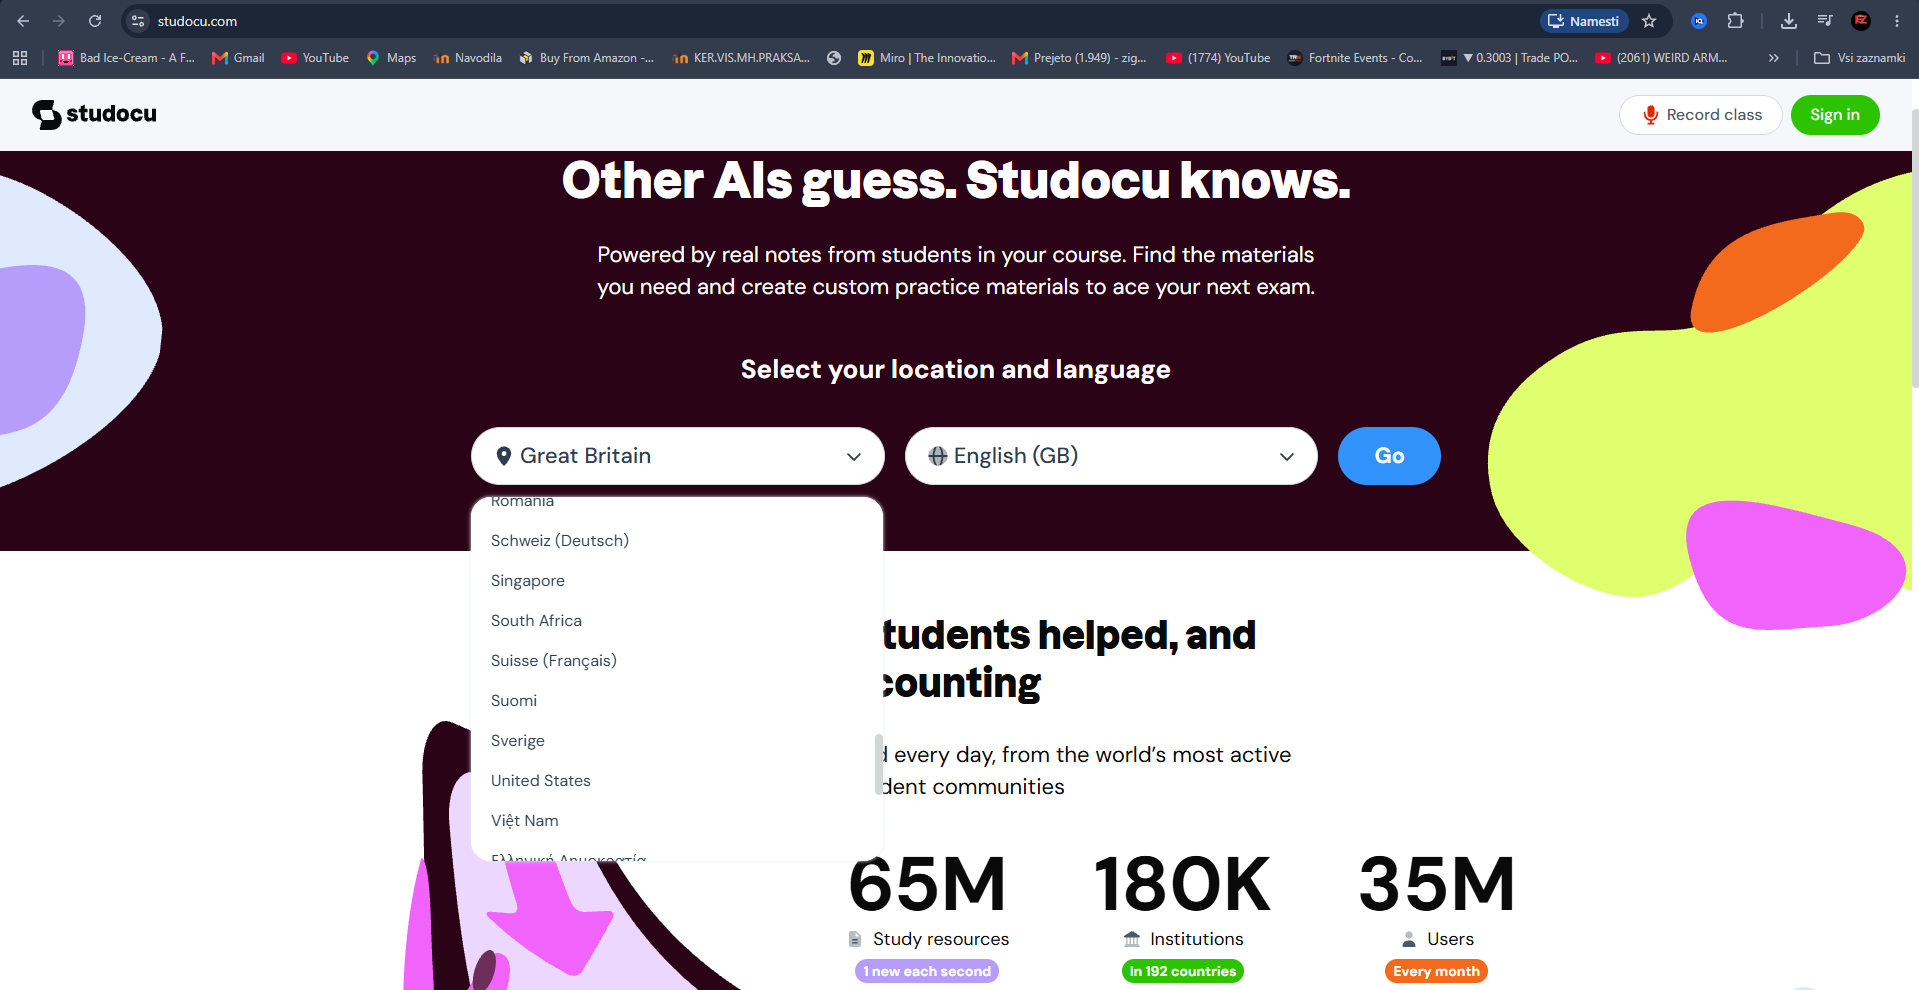
\includegraphics[width=0.85\textwidth]{studocu.png}
    \caption{Iskanje študijskih gradiv na platformi Studocu.}
    \label{fig:studocu}
\end{figure}


\subsection{Bolha.com}

\paragraph{Opis.}
Bolha.com je največji slovenski spletni oglasnik, na katerem uporabniki
objavljajo oglase za prodajo rabljenih in novih izdelkov \cite{bolha,
bolha_app}. Na voljo je kot spletna stran in mobilna aplikacija ter vsebuje
veliko kategorij, med drugim tudi knjige in učbenike.

\paragraph{Ključne funkcionalnosti.}
\begin{itemize}[noitemsep]
    \item objava oglasov s fotografijami in samodejnim predlogom kategorije,
    \item iskanje in filtriranje po kategorijah, ceni in lokaciji,
    \item shranjevanje oglasov in iskanj,
    \item sporočila med kupcem in prodajalcem,
    \item plačljivo izpostavljanje oglasov (npr.\ \emph{Skok na vrh},
          \emph{Izpostavljen oglas}) \cite{bolha_app}.
\end{itemize}

\paragraph{Prednosti.}
\begin{itemize}[noitemsep]
    \item zelo veliko uporabnikov v Sloveniji, zato je ponudba velika,
    \item slovenski jezik in lokalna usmerjenost (osebni prevzem),
    \item preprosta objava oglasov.
\end{itemize}

\paragraph{Slabosti.}
\begin{itemize}[noitemsep]
    \item ni prilagojena študentom: ni filtriranja po fakulteti, smeri ali
          predmetu,
    \item uporabniki niso preverjeni, zato obstaja tveganje prevar,
    \item ne podpira izposoje, ampak samo prodajo,
    \item ne omogoča deljenja digitalnih zapiskov.
\end{itemize}

\begin{figure}[H]
    \centering
    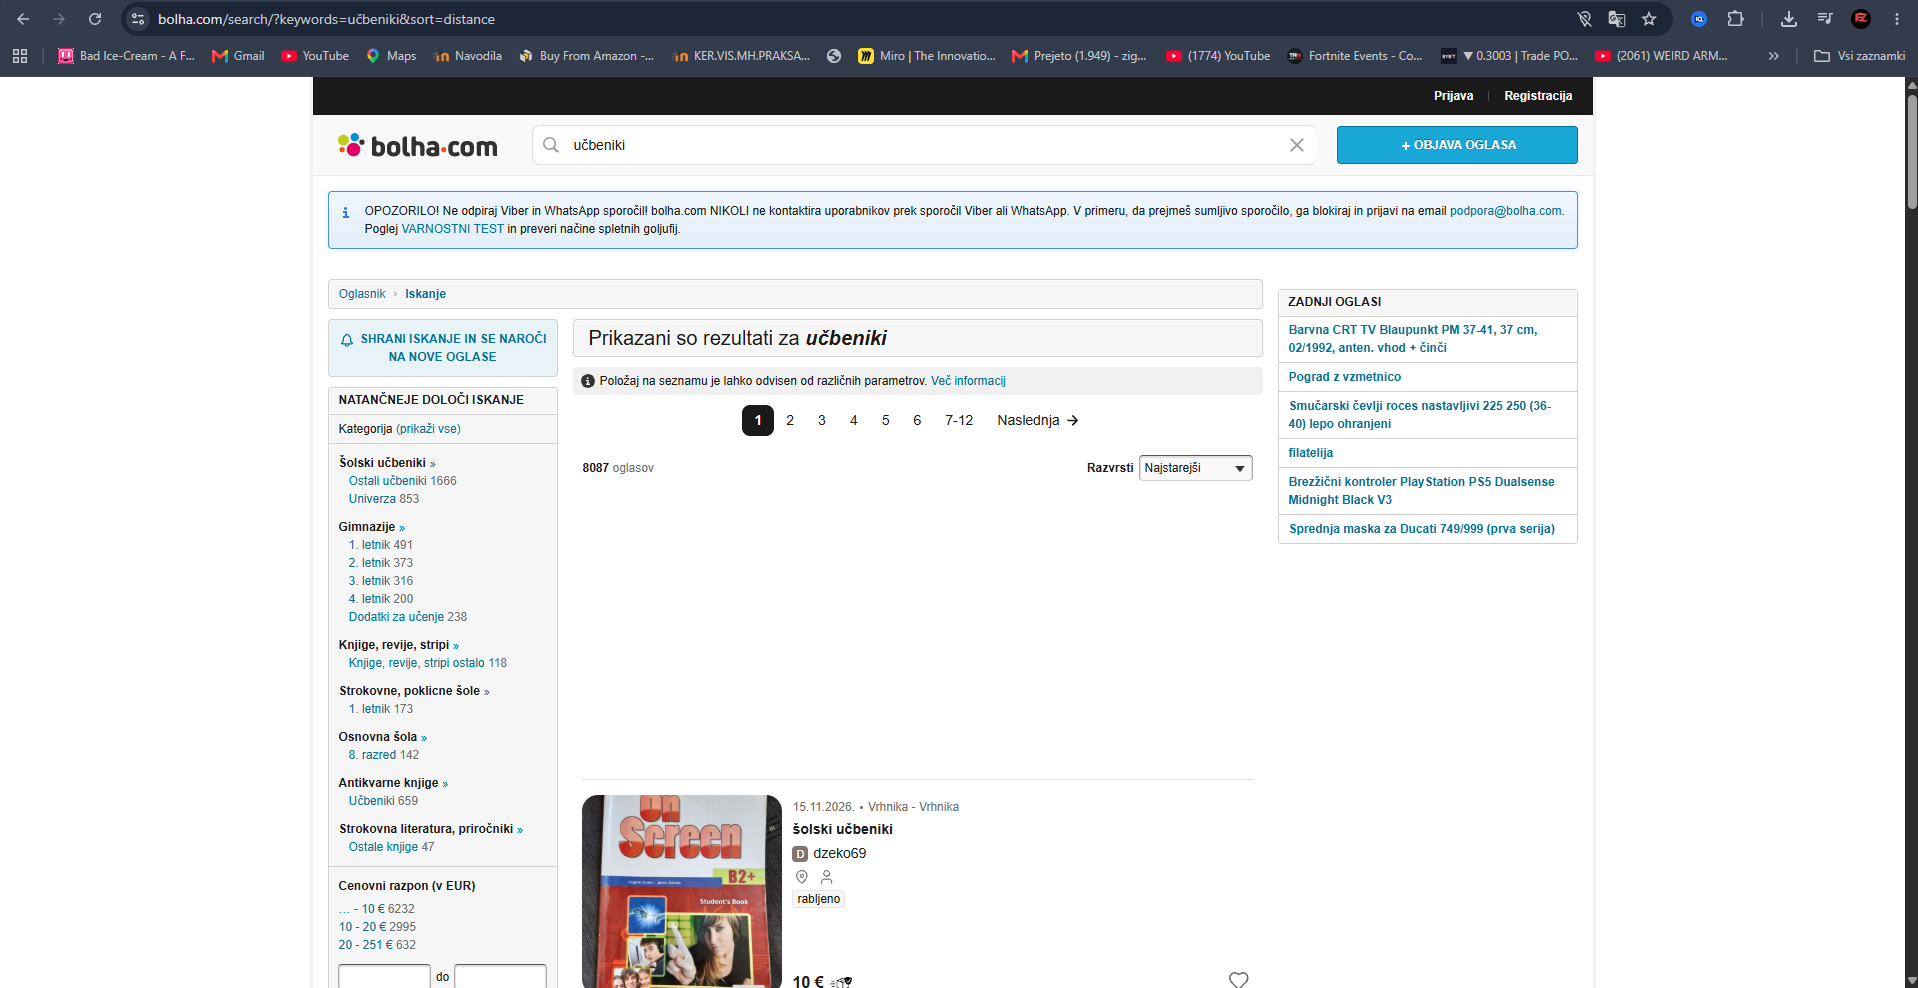
\includegraphics[width=0.85\textwidth]{bolha.png}
    \caption{Seznam oglasov v kategoriji učbenikov na oglasniku Bolha.com.}
    \label{fig:bolha}
\end{figure}


\subsection{Vinted}

\paragraph{Opis.}
Vinted je mednarodna platforma za nakup in prodajo rabljenih izdelkov med
posamezniki, ki deluje tudi v Sloveniji \cite{vinted, vinted_si}. Prvotno je
bila usmerjena v oblačila, danes pa vsebuje tudi kategorije, kot so knjige,
elektronika in hobiji.

\paragraph{Ključne funkcionalnosti.}
\begin{itemize}[noitemsep]
    \item objava izdelkov brez provizije za prodajalca,
    \item plačilo znotraj aplikacije in organizirano pošiljanje,
    \item zaščita kupca (\emph{Buyer Protection}), ki jo plača kupec ob
          nakupu \cite{vinted_fee},
    \item ocene uporabnikov po zaključenem nakupu,
    \item sporočila med kupcem in prodajalcem.
\end{itemize}

\paragraph{Prednosti.}
\begin{itemize}[noitemsep]
    \item varno plačilo in zaščita kupca zmanjšata možnost prevar,
    \item sistem ocen gradi zaupanje med uporabniki,
    \item sodobna in pregledna mobilna aplikacija.
\end{itemize}

\paragraph{Slabosti.}
\begin{itemize}[noitemsep]
    \item kupec plača dodatno pristojbino za zaščito in poštnino, kar nakup
          podraži \cite{vinted_fee},
    \item ni namenjena študentom in nima študijskih kategorij,
    \item ne podpira izposoje niti deljenja zapiskov.
\end{itemize}

\begin{figure}[H]
    \centering
    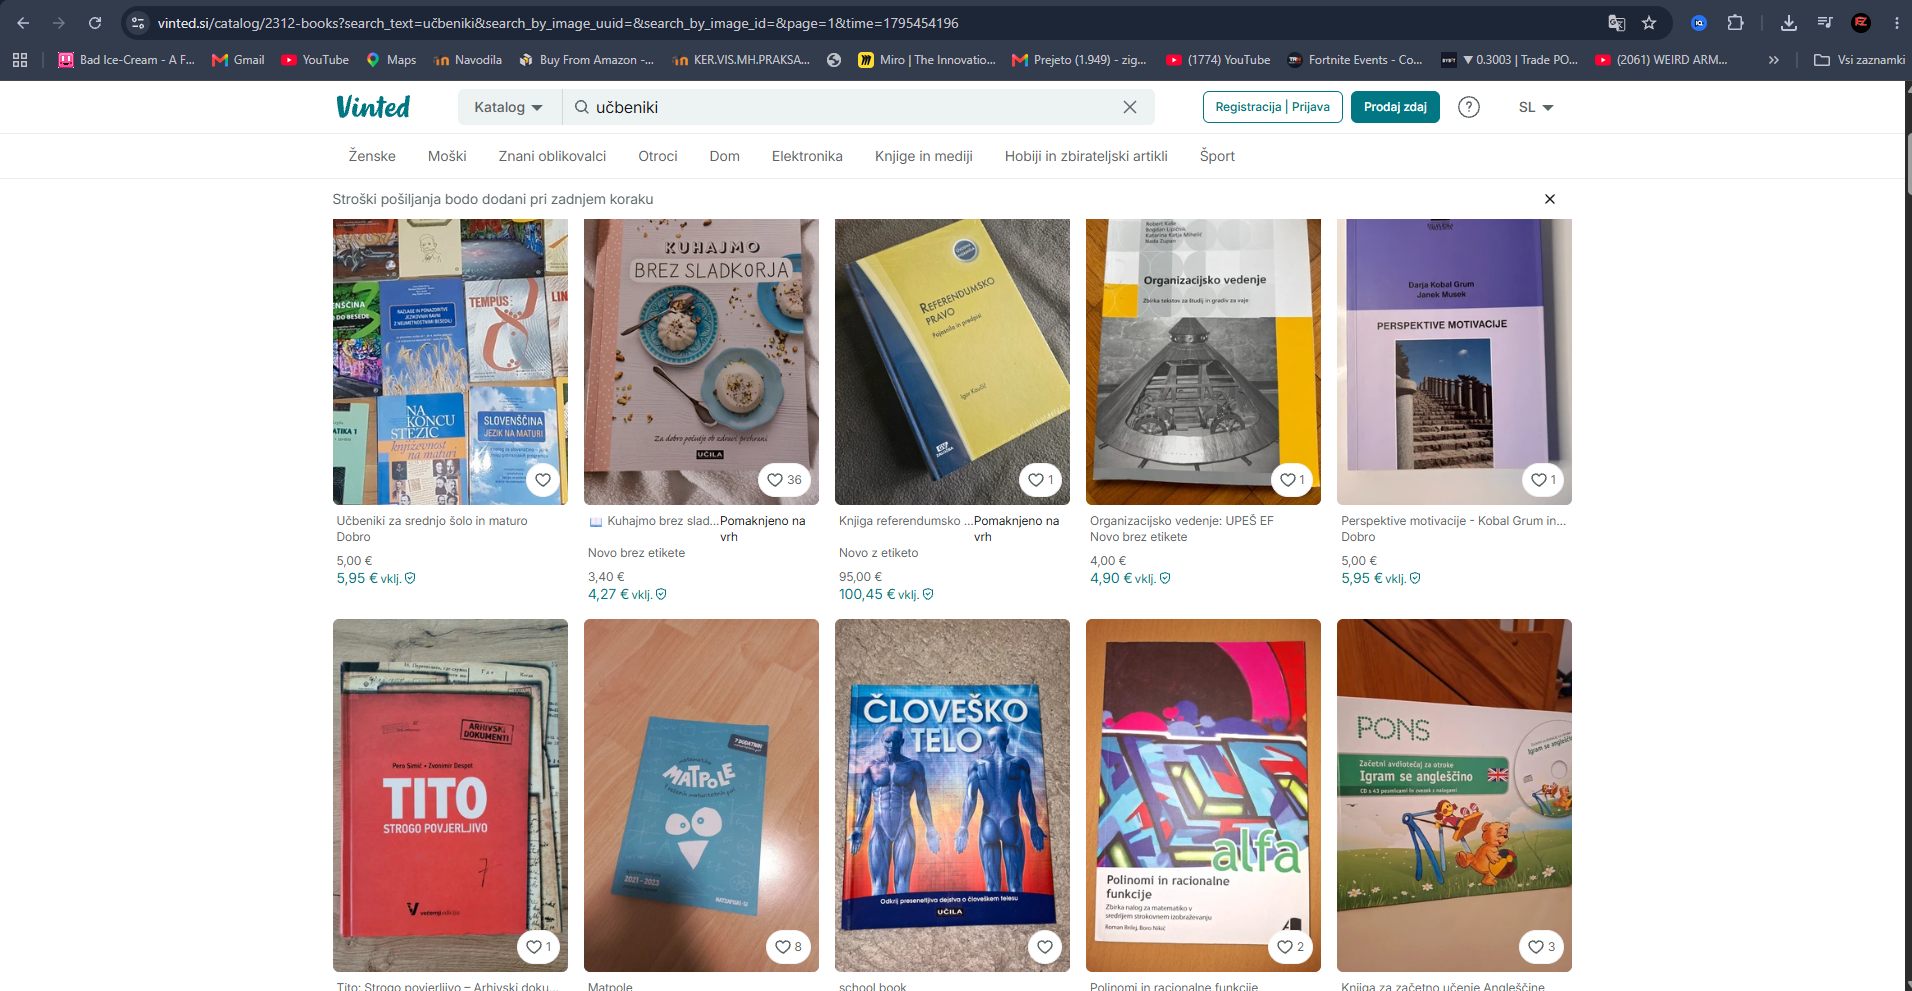
\includegraphics[width=0.85\textwidth]{vinted.png}
    \caption{Prikaz izdelka in nakupa na platformi Vinted.}
    \label{fig:vinted}
\end{figure}


\section{Primerjava rešitev}


\begin{table}[H]
\centering
\begin{tabular}{lcccc}
\hline
\textbf{Funkcionalnost} & \textbf{Studocu} & \textbf{Bolha.com} &
\textbf{Vinted} & \textbf{CampusShare} \\
\hline
Deljenje zapiskov            & da  & ne  & ne  & da \\
Prodaja opreme               & ne  & da  & da  & da \\
Izposoja opreme              & ne  & ne  & ne  & da \\
Filter po fakulteti/predmetu & da  & ne  & ne  & da \\
Preverjeni uporabniki        & ne  & ne  & delno & da \\
Ocene uporabnikov            & ne  & ne  & da  & da \\
Klepet                       & ne  & da  & da  & da \\
Koledar prevzema/vračila     & ne  & ne  & ne  & da \\
\hline
\end{tabular}
\caption{Primerjava funkcionalnosti obstoječih rešitev in projekta
CampusShare.}
\label{tab:primerjava}
\end{table}


\section{Zaključek}

Pregled je pokazal, da vsaka od obstoječih rešitev dobro pokriva le del
problema. Studocu je dober za zapiske, vendar ne omogoča izmenjave fizične
opreme. Bolha.com in Vinted omogočata prodajo, vendar nista prilagojena
študentom.

\paragraph{Kaj bomo prevzeli.}
\begin{itemize}[noitemsep]
    \item od Studocu: organizacijo gradiv po fakultetah in predmetih ter
          ocenjevanje koristnosti zapiskov,
    \item od Bolha.com: preprosto objavo oglasov in lokalni osebni prevzem,
    \item od Vinted: sistem ocen uporabnikov po zaključeni transakciji ter
          klepet med kupcem in prodajalcem.
\end{itemize}

\paragraph{Kaj bo CampusShare naredil drugače ali bolje.}
\begin{itemize}[noitemsep]
    \item združil bo zapiske in fizično opremo v eni aplikaciji,
    \item poleg prodaje bo podpiral tudi \textbf{izposojo} z zahtevki,
          potrjevanjem in koledarjem za prevzem in vračilo,
    \item dostop bo namenjen samo \textbf{preverjenim študentom} slovenskih
          fakultet, kar zmanjša možnost prevar,
    \item filtriranje bo potekalo po fakulteti, smeri in predmetu,
    \item administratorji bodo obravnavali prijave zlorab in neustreznih
          oglasov,
    \item uporaba bo za študente brezplačna oziroma cenejša kot pri
          obstoječih platformah.
\end{itemize}


\begin{thebibliography}{9}


\bibitem{studocu}
Studocu B.V., \emph{Studocu -- spletna platforma za deljenje študijskih
gradiv}. Dostopno na: \url{https://www.studocu.com} [dostopano 18.~11.~2026].

\bibitem{studocu_app}
Apple App Store, \emph{Studocu: Notes \& Practice}. Dostopno na:
\url{https://apps.apple.com/app/id1460235511} [dostopano 18.~11.~2026].

\bibitem{sme_studocu}
Save My Exams, \emph{Studocu vs Save My Exams: Full Comparison}. Dostopno na:
\url{https://www.savemyexams.com/learning-hub/sme-articles/save-my-exams-vs-studocu/}
[dostopano 18.~11.~2026].

\bibitem{bolha}
Bolha.com, \emph{Spletni oglasnik Bolha.com}. Dostopno na:
\url{https://www.bolha.com} [dostopano 18.~11.~2026].

\bibitem{bolha_app}
Apple App Store, \emph{bolha.com}. Dostopno na:
\url{https://apps.apple.com/si/app/bolha-com/id1540081488}
[dostopano 18.~11.~2026].

\bibitem{vinted}
Vinted, \emph{Vinted -- platforma za nakup in prodajo rabljenih izdelkov}.
Dostopno na: \url{https://www.vinted.si} [dostopano 18.~11.~2026].

\bibitem{vinted_si}
The Slovenia, \emph{Vinted Slovenia 2026: How to Buy, Sell and Send
Packages}. Dostopno na: \url{https://the-slovenia.com/en/lifestyle/vinted-slovenia/}
[dostopano 18.~11.~2026].

\bibitem{vinted_fee}
Vinted, \emph{Buyer Protection fee on Vinted}. Dostopno na:
\url{https://www.vinted.co.uk/help/342} [dostopano 18.~11.~2026].

\end{thebibliography}

\end{document}